
\section{Working with Other Providers of Scientific Infrastructure to Improve Support for Documenting Provenance and Replicability}
\label{sec:coordination}

An important responsibility of the AEA Data Editor is to interact with other providers of scientific infrastructure. This includes other publishers and journals, archives such as ICPSR, providers of restricted or proprietary data, metadata harvesters, and third-party verification services. 


\subsection{AEA RCT Registry}
\label{sec:registry}

The \rctr{} (Registry) provides services to the economics (and social science) community at large. Managed at J-PAL and funded by the AEA, registration at the Registry is mandatory for field experiments published in \ac{AER}, \ac{AERI}, \ac{AEJAPP}, and \ac{AEJPOL}, but is also used more broadly in the economics discipline, with numerous publications in top economics journals as well as field journals identifying pre-registration in the Registry. The Registry is available at \href{https://www.socialscienceregistry.org/}{www.socialscienceregistry.org}.\footnote{This section is based in part on information provided by Stuti Goyal, Jack Cavanagh, and Sarah Kopper. All errors are mine.}
%
In collaboration with members of the AEA's \textit{Oversight Committee for Registry of Random Controlled Trials}, the Registry team at J-PAL have continued to work on improving the usability of the Registry, as well as ensuring the availability of Registry data. 


Data for the Registry is being curated and preserved in the \textit{AEA RCT Registry Dataverse} at 
\href{https://dataverse.harvard.edu/dataverse/aearegistry}{dataverse.harvard.edu/dataverse/aearegistry}, allowing for reproducible analysis of the universe of registrations by researchers.%
\footnote{Data shown in this report are derived from \citet{DVN/2RZF2X_2024}, and show data for calendar year \reportyear{}.  
%End-of-year numbers for \reportyear{} were extrapolated based on data from the first 11 months of \reportyear{}, as of \lastday{}. 
} 

% The Data Editor monitors proper reference to and citation of registrations. A registration should be cited in the text and the title footnote as, for example, ``\textit{Zhang (2017)}'' (the title footnote should also mention ``\textit{AEARCTR-0000005}''), and the references should have the appropriate entry:

% \begin{quote}\footnotesize
%     Zhang, Kelly. 2017. "Voter Pessimism and Electoral Accountability: Experimental Evidence from Kenya." AEA RCT Registry. May 02. https://doi.org/10.1257/rct.5-8.0.
% \end{quote}

%{\color{red}Additional data to come.}

%While the AEA journals mentioned above remain among the few economics journals that strictly require registration, 
Usage of the registration continues to increase strongly. As Figures~\ref{fig:registry1} and~\ref{fig:registry2} show, the rate of registrations per year continues to rise, and the registry now has over \regscumul{} registrations, which are being added at a rate of \regsyearly{} per year.  More than \registeredusers{} unique researchers are associated with these registrations (left panel, Figure~\ref{fig:registry2}), \activeusers{} of which are associated with registrations that have been active in \reportyear{}. The share of pre-registrations, favored by some, surpassed post-registrations for the first time in 2021, and remains higher (right panel, Figure~\ref{fig:registry2}). 

% src=https://github.com/J-PAL/AEA_registryanalysis/archive/refs/heads/main.zip

\begin{figure}
\centering
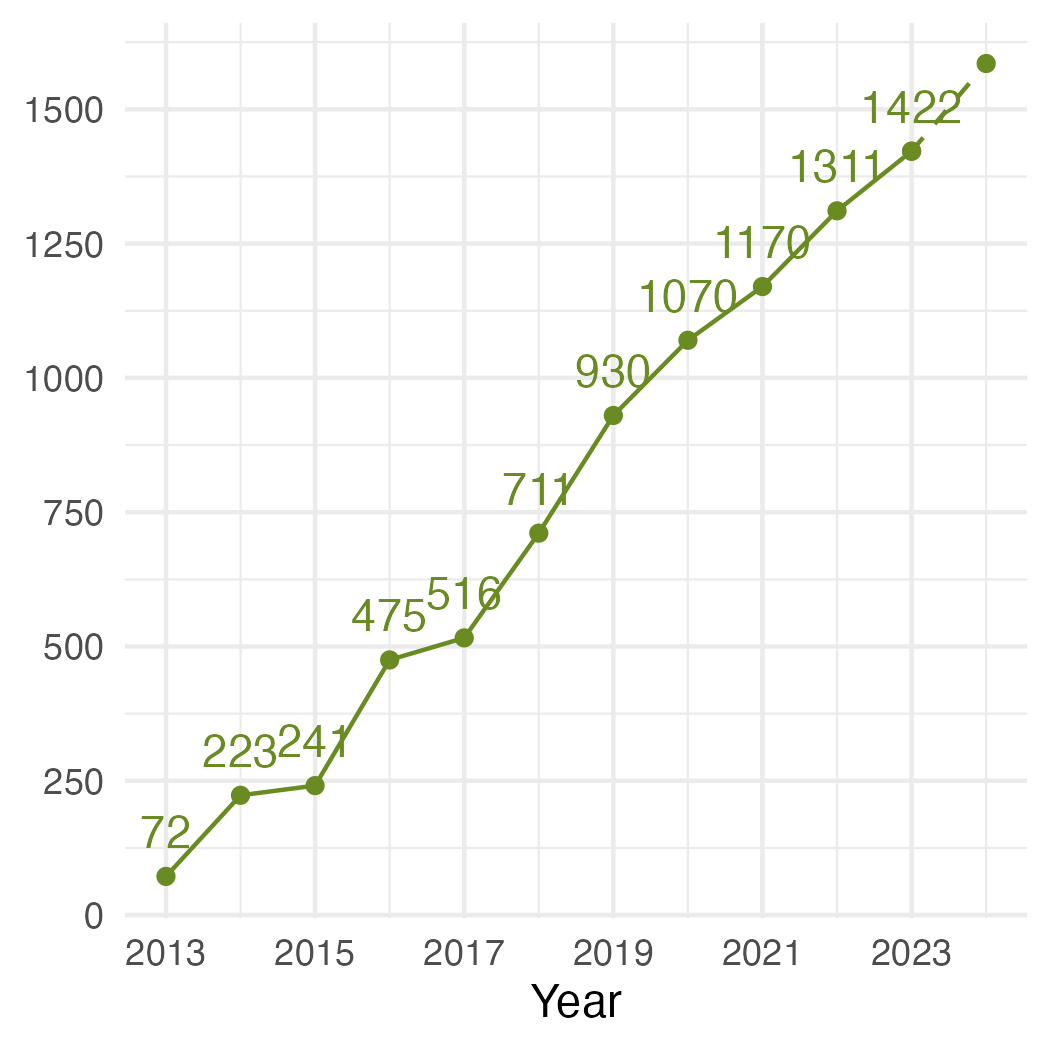
\includegraphics[width=0.4\textwidth]{data/registry/Output/reg_pre_year_2023.png}
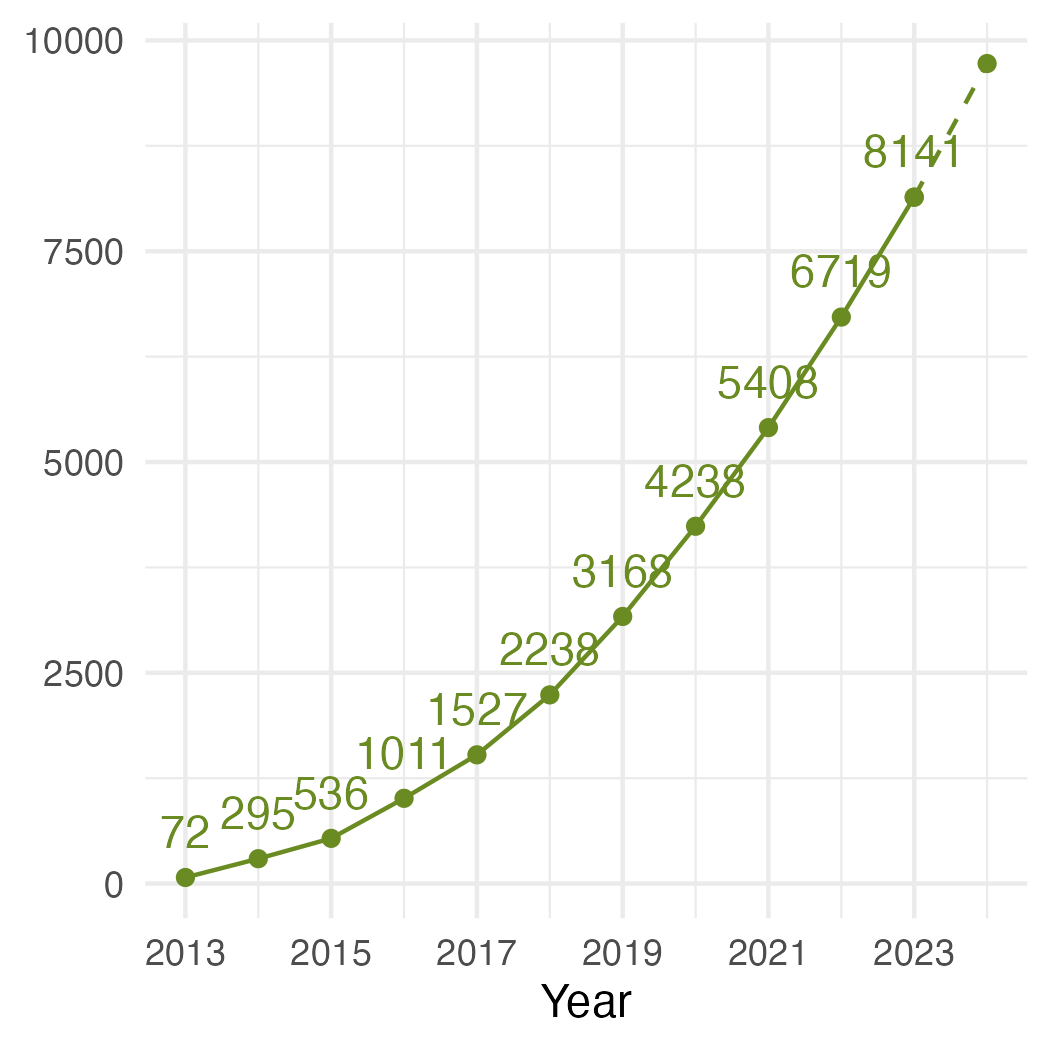
\includegraphics[width=0.4\textwidth]{data/registry/Output/reg_cumulative_2023.png}
\caption{Annual (left) and Cumulative Registrations (right) }
    \label{fig:registry1}
\caption*{\footnotesize Source: \citet{DVN/2RZF2X_2024}. Dashed lines are extrapolated increases for 2024.}
\end{figure}

\begin{figure}
\centering
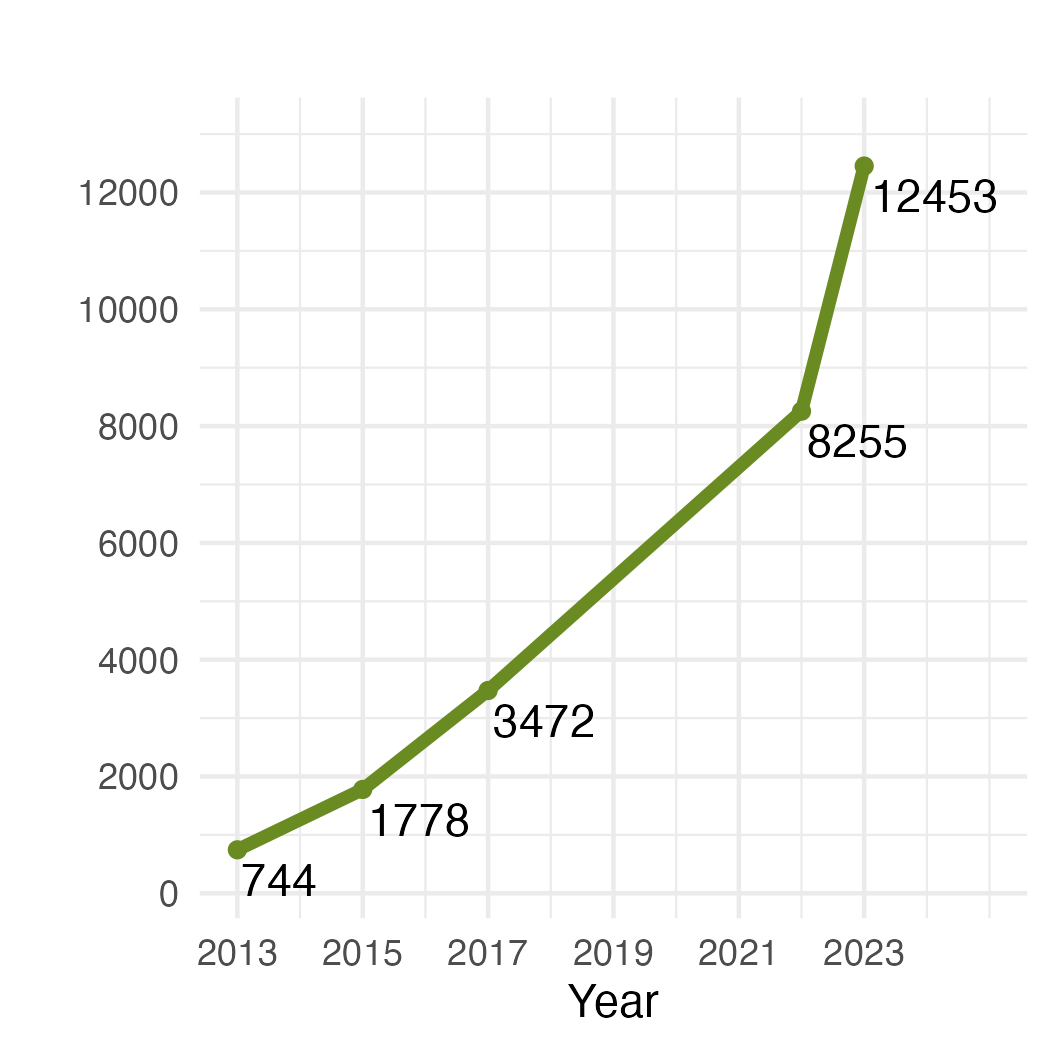
\includegraphics[width=0.4\textwidth]{data/registry/Output/registered_users_2023.png}
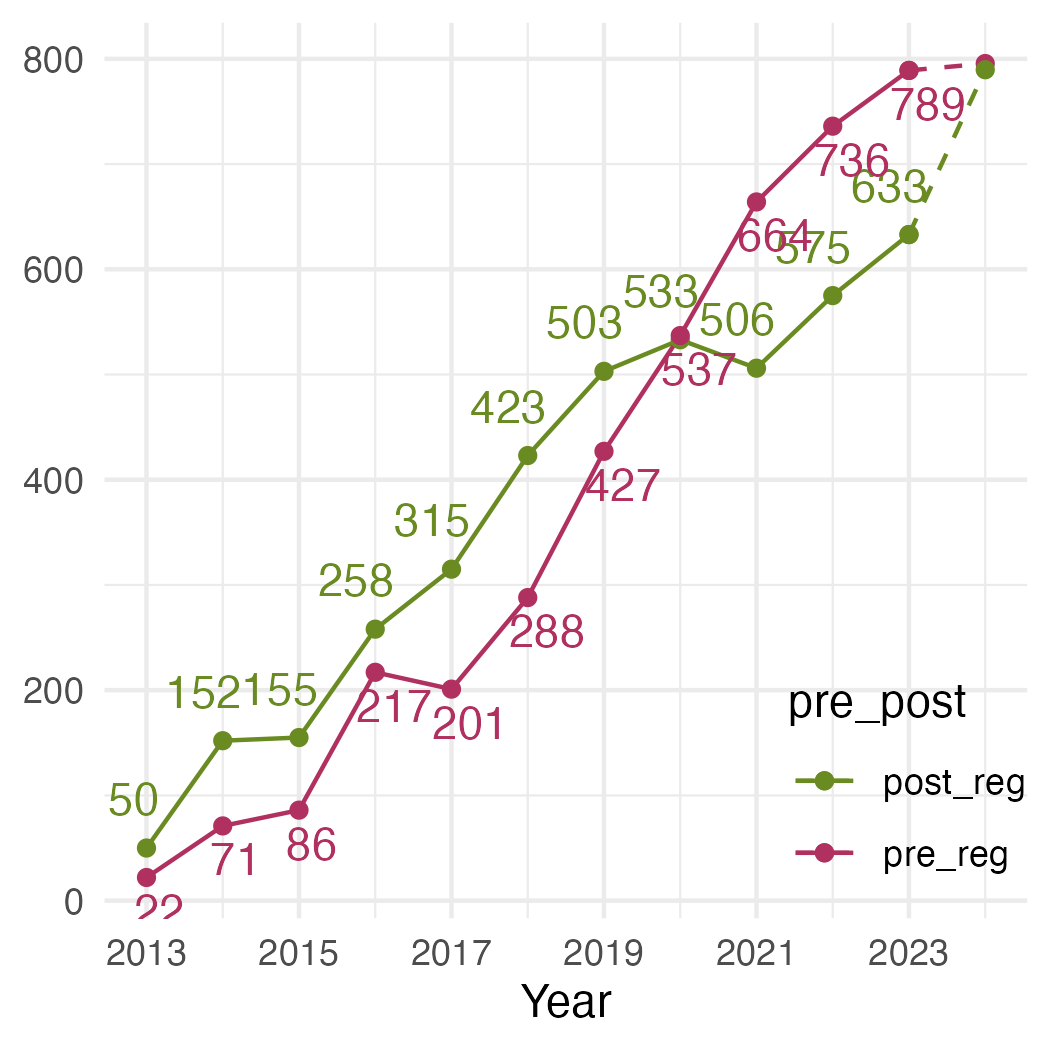
\includegraphics[width=0.4\textwidth]{data/registry/Output/post_pre_reg_2023.png}
\caption{Unique registered investigators (left), Post vs Pre-registrations (right)}
    \label{fig:registry2}
\caption*{\footnotesize Source: \citet{DVN/2RZF2X_2024}. Dashed lines are extrapolated increases for 2024.}
\end{figure}

As the registry has continued to grow, attract new users, and become a standard for experiments across economics and related social sciences, it is improving in its function as a central database of those experiments. In the last five years, an increasing number of articles  use the publicly available registry metadata as either their main analysis data or as a supplement to it. These can be grouped into a few broad sets.  
%
% In particular, multiple published articles and working papers use the Registry to analyze the scientific aspects of (pre-)registration, see \citet{corduneanu-huci_what_2022,
% miguel_evidence_2021,
% murtagh-white_learning_2023,
% leight_publication_2022,
% christensen_open_2019,
% ofosu_pre-analysis_2019,
% laitin_reporting_2021,
% abrams_research_2020,
% corduneanu-huci_politics_2021,
% buckley_role_2022,
% christensen_transparency_2018}.
%
%
One group of papers use the registry to study research transparency questions in the social sciences, either studying the registry as a transparency object in itself \citep{christensen_transparency_2018,abrams_research_2020,miguel_evidence_2021}, taking it as a means to glean information on other transparency behaviors \citep{ofosu_pre-analysis_2019,laitin_reporting_2021}, or  using it as an auditing tool, both for self-reported data \citep{christensen_open_2019} and the implementation of transparency policies \citep{buckley_role_2022}. A second group use the registry data as a significant portion of a larger compiled dataset attempting to proxy for the universe of experiments and experimenters in a particular subset of social science research \citep{corduneanu-huci_politics_2021,corduneanu-huci_what_2022}. A last group of studies use the data to answer meta-scientific questions about the studies on the registry \citep{leight_publication_2022,murtagh-white_learning_2023}.


% \subsection{Highlighting and Preserving Data Resources}

% We identified Zenodo as a possible solution to preserving large-scale data resources that surpass the practical capabilities of the \aeadcr{}. By creating the ``AEA Zenodo Community,'' we are able to highlight data resources that have, in the past, often not been curated or preserved appropriately. For instance, \citet{u_s_geological_survey_2022_5830968} comprises 83GB of data, preserved from DVDs and complemented and corrected manually based on online sources. They constitute some of the input data for \citet{10.1257/app.20200398}. Similarly, \citet{ministerio_de_desarrollo_productivo_arge_2022_6568295} preserves 44 GB of daily price data  captured in 2016-2018 and used by \citet{10.1257/mac.20210172}. In both cases, the data are under liberal licenses (public domain or Creative Commons licenses), which allow for the republication of the data. 


\subsection{Data Providers}
\label{sec:producers}

We regularly meet and communicate with academic, governmental, and commercial data providers, on behalf of specific authors or because we have identified a data provider as a frequently used resource. Discussion topics include making data citations easier, clarifying licenses, requesting blanket or streamlined data redistribution or access authorizations, or suggesting improved data curation practices to avoid repeatedly copying data from uncurated websites to the curated \aeadcr{}. 

In the course of the past year, we have talked about some or all of these topics with IPUMS, the World Bank (see also below), staff at the U.S. Census Bureau, the \ac{IRS}, the \ac{BLS}, the (German) Institute for Employment Research (IAB),  the \ac{BPLIM},  and the French \textit{Centre d'accès sécurisé de données} (CASD). We have also talked to various research groups on how to improve data curation, visibility, and citability of the data created by their efforts. 

\subsection{Economics Journals}

We continue to coordinate with other data editors conducting similar activities at other journals. An informal mailing list managed by the AEA Data Editor is used to interact with others.\footnote{Journal editors are encouraged to join the mailing list by contacting the AEA Data Editor.} Mailing list members who wish to be more actively involved can join the \textbf{monthly video call}, and participate in the development of the \purlcite{socialsciencedataeditors.github.io}{website of the Social Science Data Editors} In addition to the Data Editor of the AEA, the current group includes Miklós Koren (Data Editor, \acl{ReStud}), Florian Oswald (Data Editor, \acl{EJ} and Econometric Journal), Joan Llull (Data Editor, Econometrica),  Marie Connolly (Data Editor, \acl{CJE}), Anna Dreber Almenberg (Editor, JPE Microeconomics), and Maia G\"uell (Data Editor, \acl{JEEA}).  The website contains guidance on data citations and data availability statements, best practices for coding and data preparation, and links to various tools useful to replicators. In particular, the group coordinates the \textit{Template README} \citep{READMEv1.1.0}, which was last updated in November 2022, and which is referenced as a \textit{common} reference implementation for providing required information  across a number of journals. Furthermore, the group has developed a common standard for replication packages (\ac{DCAS}), which journals can use to signal that their requirements are similar to those commonly required by all endorsers of the standard \citep{datacodestandardv1}.%
\footnote{
After the 2024 Annual Meetings, but before final copy-editing for this report, the AEA's \acf{DCAP} was updated to conform to the order, format, and content of the \ac{DCAS}, see \href{https://www.aeaweb.org/journals/data/data-code-policy}{aeaweb.org/journals/data/data-code-policy}. The update does not change any requirements. The previous version of the policy can be found at \href{https://www.aeaweb.org/journals/data/archive/2020-2024}{aeaweb.org/journals/data/archive/2020-2024}. } 
%
Joint presentations and tutorials by the group involving the AEA Data Editor include the aforementioned presentations and workshops in Montréal (with Connolly), at the RES (with Connolly) and the EEA (with Koren).
%
The AEA Data Editor  also coordinates with the Editor and Data Editor of Economic Inquiry, and has had discussions with other editors and data editors seeking in put on their practices and policies. He furthermore participates in  the Steering Committee of a group of data repository leaders at Data-PASS organized as the Journal Editors Discussion Interface \purlcite{https://dpjedi.org/}{({JEDI})}


\subsection{Third-party verification services}
\label{sec:3rdparty}


We continue to rely on and have discussions with third-party verification services. As noted earlier, \jiraexternal{} reports were provided by external replicators or replication services
%for \jiramcsexternal{} manuscripts 
(see Table~\ref{tab:jirastats} for statistics by journal, and Appendix~\ref{app:3rdparty} for a list of third-party replicators). Of note, the World Bank has introduced a reproducibility \curlcite{https://reproducibility.worldbank.org/index.php/about}{verification service} which ``[verifies packages] to ensure that they are complete and fully functional before they are published to the repository.'' We will accept such third-party verifications, both at the time of submission as well as upon request, as long as the process by which they are created is documented and consistent with the approach that the economics journals are using. We are working on a mechanism to robustly  \purlcite{https://transparency-certified.github.io/}{``certify'' such processes}

\section{Working with the Economics Community to Enhance and Broaden Education on Replicable Science}

Outreach through presentations and publicly available tools is a key component of an effective data and code availability policy. 
%
Recordings of  presentations (when available) and presentation materials are listed at the \purlcite{https://aeadataeditor.github.io/talks/}{Data Editor's website} In addition to presentations, the Data Editor occasionally is an observer at \curlcite{https://i4replication.org/description.html}{Replication Games} where teams of researchers and students attempt to reproduce and extend papers published in leading economics journals. Such post-publication verifications are a necessary and useful check on published replication packages. Replicators may find issues that were not discovered, or discoverable, by pre-publication replicators such as the AEA Data Editor team. The Data Editor facilitates and monitors that any corrections or suggested improvements are conveyed to authors, and are reflected on replication packages via the AEA's \textit{Policy on Revisions of Data and Code Deposits} (see Appendix~\ref{sec:list-of-policies}). Several such (minor) corrections have lead to updates (see Table~\ref{tab:updates}). 
%


\subsection{Resources}

The AEA Data Editor maintains public resources available to the economics community. These are made available through a dedicated website at \href{https://aeadataeditor.github.io/}{aeadataeditor.github.io/} and code and project templates provided at \href{https://github.com/aeadataeditor}{github.com/aeadataeditor}. In particular:

\begin{itemize}
    \item Step-by-step guidance on how to prepare a replication package is provided at \href{https://aeadataeditor.github.io/aea-de-guidance/}{aeadataeditor.github.io/aea-de-guidance/}, including video tutorials and a description of the process. 
    \item The template README \citep{READMEv1.1.0} is referenced as part of the guidance, and separately accessible at \href{https://social-science-data-editors.github.io/template_README/}{social-science-data-editors.github.io/template\_README/}.
    \item Various blog posts on topics relating to computational reproducibility are posted at \href{https://aeadataeditor.github.io/year-archive/}{aeadataeditor.github.io/year-archive/}, and may be summarized on Twitter under the Data Editor's handle \href{https://twitter.com/AEAData}{@AEAData},  on Mastodon under \href{https://mstdn.social/@aeadata}{@aeadata@mstdn.social}, and on BlueSky under \href{https://bsky.app/profile/aeadata.bsky.social}{@aeadata.bsky.social}
    \item Instructions to replicators for assessing authors' replication packages are provided at \href{https://github.com/AEADataEditor/replication-template}{github.com/AEADataEditor/replication-template}.
    \item Template code for using containers for Stata, R, Julia, and Gurobi can be found by \href{https://github.com/AEADataEditor?q=docker&type=all&language=&sort=}{searching for ``docker`` on the Github site}.
    
\end{itemize}
